\documentclass[a4paper,12pt]{article}
\usepackage[utf8]{inputenc}
\usepackage{graphicx}
\usepackage{amsmath}
\usepackage{booktabs}
\usepackage{caption}
\usepackage{subcaption}
\usepackage{geometry}
\geometry{margin=1in}

\title{Analisi Comparativa di Due Run di Valutazione Basate su BERT per l'Integrità dell'Allineamento di Testi Generati da LLM}
\author{[Bianchi Francesco, Brighenti Stefano]}
\date{\today}

\begin{document}

\maketitle


\section{Introduzione}
L'integrità dell'allineamento dei modelli linguistici di grandi dimensioni (LLM) è cruciale per il loro utilizzo etico e sicuro. Questo studio confronta due run di valutazione basate su BERT per identificare violazioni dell'allineamento nei testi generati. La Run 1 utilizza BERT base senza fine-tuning, mentre la Run 2 applica un fine-tuning su un dataset di risposte simili. Il dataset comune consta di 1784 istanze, con 997 etichettate come "no break" (0) e 787 come "break" (1). L'obiettivo è valutare l'impatto del fine-tuning sulla capacità di classificazione e clustering.

\section{Metodologia}
Le due run sono state condotte in un ambiente Colab con codice identico, differendo solo per il modello BERT:
\begin{itemize}
\item \textbf{Run 1}: BERT base non fine-tuned.
\item \textbf{Run 2}: BERT base fine-tuned su un dataset di risposte simili.
\end{itemize}

Il dataset di 1784 testi è stato analizzato con k-means per il clustering, determinando il numero ottimale di cluster (\(k\)) tramite i metodi elbow e silhouette. Sono state generate visualizzazioni PCA e t-SNE per rappresentare i macro-cluster e i sottocluster. Le matrici di confusione sono state costruite confrontando le etichette predette con quelle reali.

\section{Risultati}

\subsection{Run 1: BERT Non-Tuned}
I risultati della Run 1 includono:
\begin{itemize}
\item \textbf{Conteggi dei macro-cluster}:
  \begin{itemize}
  \item Cluster 0 (no-jailbreak): 331 elementi
  \item Cluster 1 (jailbreak): 1442 elementi
  \end{itemize}
\item \textbf{Matrice di confusione}: La Tabella \ref{tab:conf_run1_tot} mostra la matrice con totali.
\item \textbf{Visualizzazioni}:
  \begin{itemize}
  \item La Figura \ref{fig:run1_elbow0} mostra l'analisi elbow e silhouette per il Macro-cluster 0 (no-jailbreak).
  \item La Figura \ref{fig:run1_elbow1} mostra l'analisi elbow e silhouette per il Macro-cluster 1 (jailbreak).
  \item La Figura \ref{fig:run1_pca_tot} visualizza i macro-cluster tramite PCA.
  \item La Figura \ref{fig:run1_tsne_tot} visualizza i macro-cluster tramite t-SNE.
  \item La Figura \ref{fig:run1_pca_div} mostra i sottocluster all'interno dei macro-cluster tramite PCA.
  \item La Figura \ref{fig:run1_tsne_div} mostra i sottocluster all'interno dei macro-cluster tramite t-SNE.
  \end{itemize}
\end{itemize}

\begin{table}[h]
    \centering
    \begin{tabular}{c|cc|c}
        \toprule
        & Predetto No-Break (0) & Predetto Break (1) & Totale \\
        \midrule
        Reale No-Break (0) & 331 & 666 & 997 \\
        Reale Break (1) & 0 & 787 & 787 \\
        \midrule
        Totale & 331 & 1453 & 1784 \\
        \bottomrule
    \end{tabular}
    \caption{Matrice di confusione per la Run 1 (BERT non-tuned) con totali.}
    \label{tab:conf_run1_tot}
\end{table}

\begin{figure}[h]
    \centering
    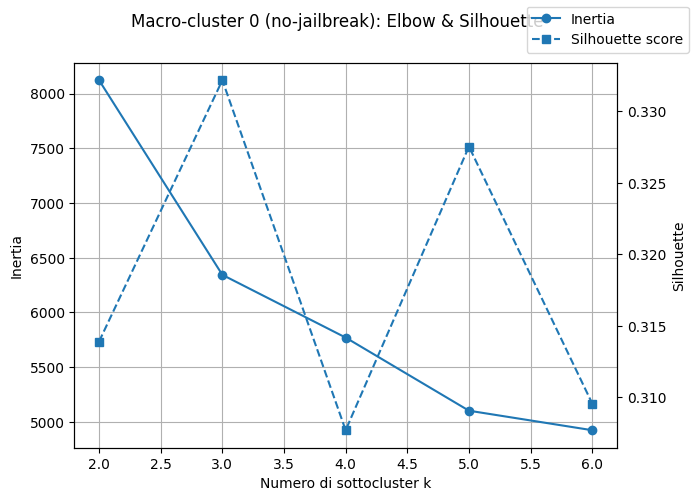
\includegraphics[width=0.8\textwidth]{run1-elbow0.png}
    \caption{Analisi elbow e silhouette per il Macro-cluster 0 (no-jailbreak) nella Run 1.}
    \label{fig:run1_elbow0}
\end{figure}

\begin{figure}[h]
    \centering
    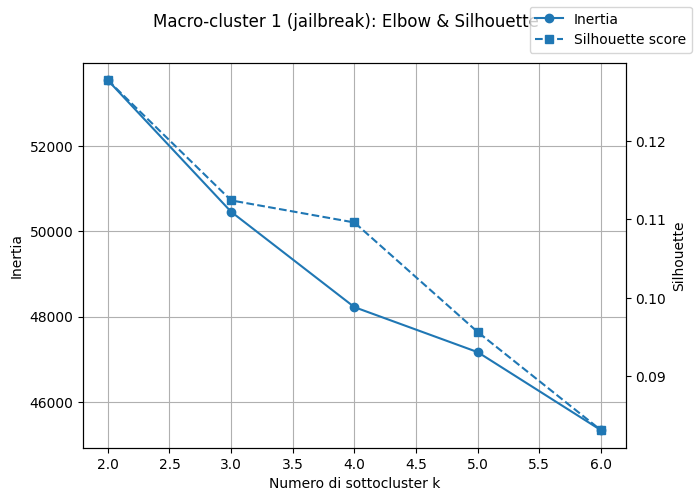
\includegraphics[width=0.8\textwidth]{run1-elbow1.png}
    \caption{Analisi elbow e silhouette per il Macro-cluster 1 (jailbreak) nella Run 1.}
    \label{fig:run1_elbow1}
\end{figure}

\begin{figure}[h]
    \centering
    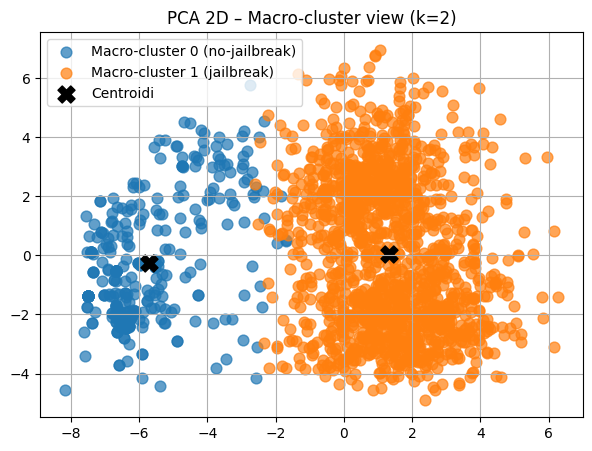
\includegraphics[width=0.8\textwidth]{run1-pca-tot.png}
    \caption{Visualizzazione PCA dei macro-cluster nella Run 1.}
    \label{fig:run1_pca_tot}
\end{figure}

\begin{figure}[h]
    \centering
    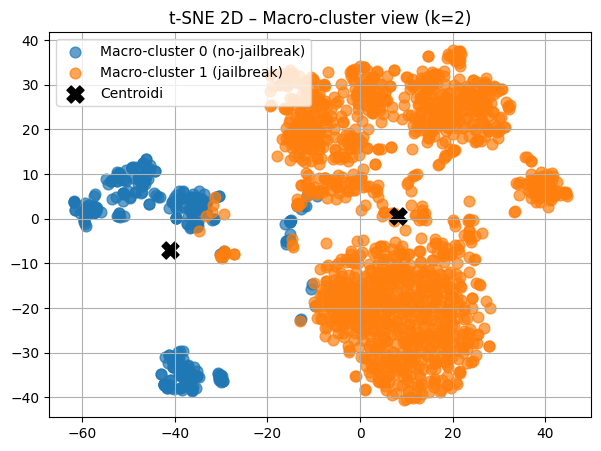
\includegraphics[width=0.8\textwidth]{run1-tsne-tot.png}
    \caption{Visualizzazione t-SNE dei macro-cluster nella Run 1.}
    \label{fig:run1_tsne_tot}
\end{figure}

\begin{figure}[h]
    \centering
    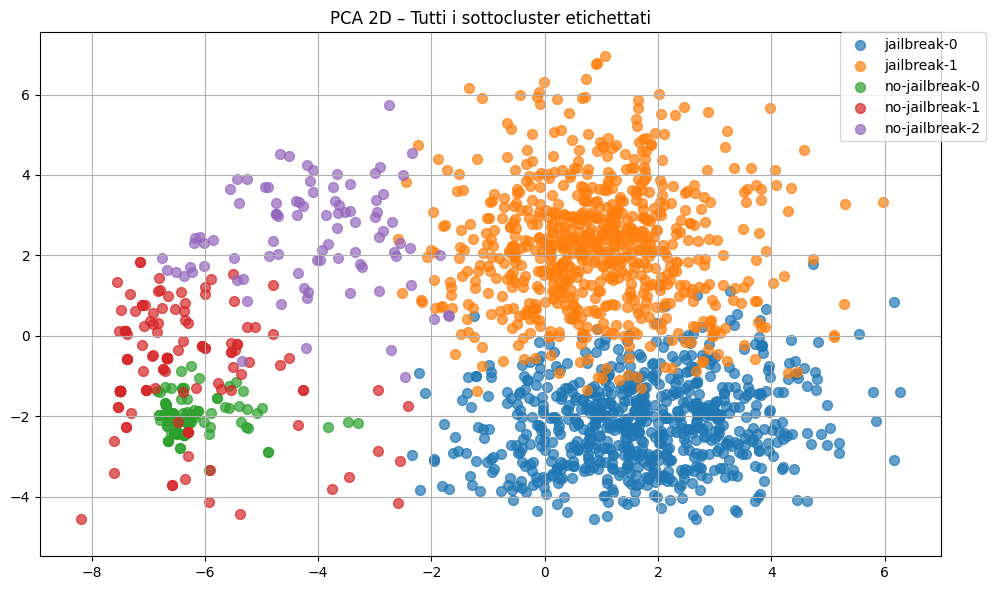
\includegraphics[width=0.8\textwidth]{run1-pca-div.png}
    \caption{Visualizzazione PCA dei sottocluster all'interno dei macro-cluster nella Run 1.}
    \label{fig:run1_pca_div}
\end{figure}

\begin{figure}[h]
    \centering
    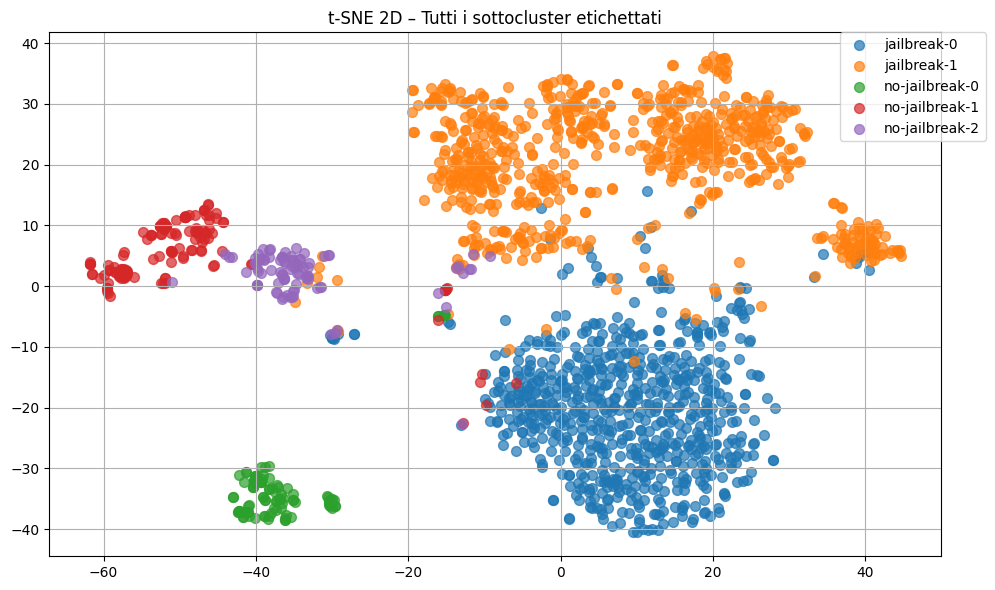
\includegraphics[width=0.8\textwidth]{run1-tsne-div.png}
    \caption{Visualizzazione t-SNE dei sottocluster all'interno dei macro-cluster nella Run 1.}
    \label{fig:run1_tsne_div}
\end{figure}

\subsection{Run 2: BERT Fine-Tuned}
I risultati della Run 2 includono:
\begin{itemize}
\item \textbf{Conteggi dei macro-cluster}:
  \begin{itemize}
  \item Cluster 0 (no-jailbreak): 1087 elementi
  \item Cluster 1 (jailbreak): 686 elementi
  \end{itemize}
\item \textbf{Matrice di confusione}: La Tabella \ref{tab:conf_run2_tot} mostra la matrice con totali.
\item \textbf{Visualizzazioni}:
  \begin{itemize}
  \item La Figura \ref{fig:run2_elbow0} mostra l'analisi elbow e silhouette per il Macro-cluster 0 (no-jailbreak).
  \item La Figura \ref{fig:run2_elbow1} mostra l'analisi elbow e silhouette per il Macro-cluster 1 (jailbreak).
  \item La Figura \ref{fig:run2_pca_tot} visualizza i macro-cluster tramite PCA.
  \item La Figura \ref{fig:run2_tsne_tot} visualizza i macro-cluster tramite t-SNE.
  \item La Figura \ref{fig:run2_pca_div} mostra i sottocluster all'interno dei macro-cluster tramite PCA.
  \item La Figura \ref{fig:run2_tsne_div} mostra i sottocluster all'interno dei macro-cluster tramite t-SNE.
  \end{itemize}
\end{itemize}

\begin{table}[h]
    \centering
    \begin{tabular}{c|cc|c}
        \toprule
        & Predetto No-Break (0) & Predetto Break (1) & Totale \\
        \midrule
        Reale No-Break (0) & 997 & 0 & 997 \\
        Reale Break (1) & 90 & 697 & 787 \\
        \midrule
        Totale & 1087 & 697 & 1784 \\
        \bottomrule
    \end{tabular}
    \caption{Matrice di confusione per la Run 2 (BERT fine-tuned) con totali.}
    \label{tab:conf_run2_tot}
\end{table}

\begin{figure}[h]
    \centering
    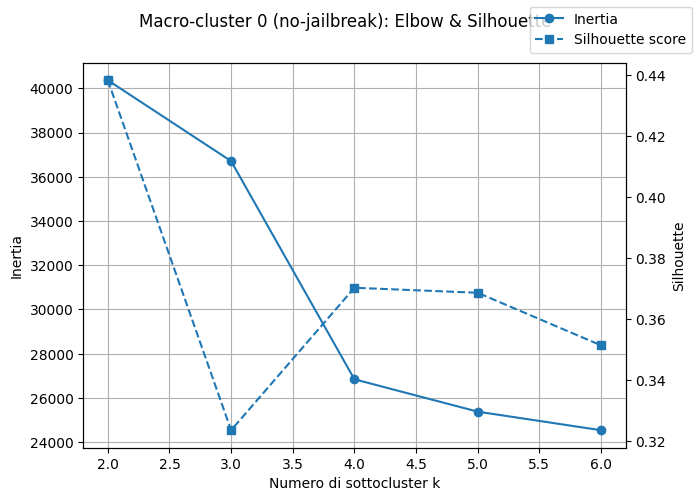
\includegraphics[width=0.8\textwidth]{run2-elbow0.png}
    \caption{Analisi elbow e silhouette per il Macro-cluster 0 (no-jailbreak) nella Run 2.}
    \label{fig:run2_elbow0}
\end{figure}

\begin{figure}[h]
    \centering
    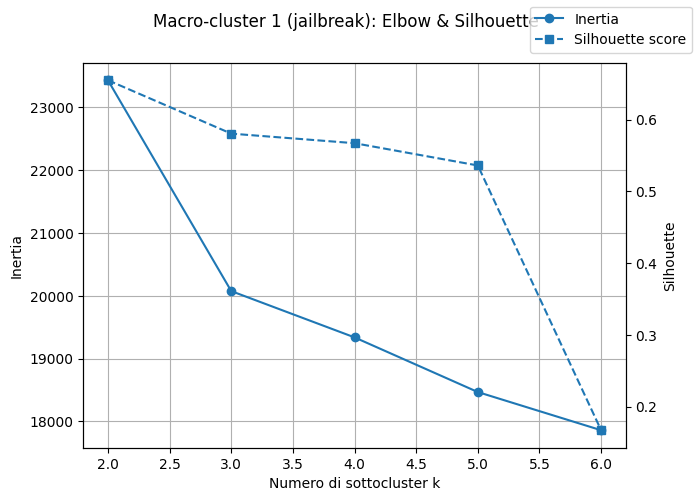
\includegraphics[width=0.8\textwidth]{run2-elbow1.png}
    \caption{Analisi elbow e silhouette per il Macro-cluster 1 (jailbreak) nella Run 2.}
    \label{fig:run2_elbow1}
\end{figure}

\begin{figure}[h]
    \centering
    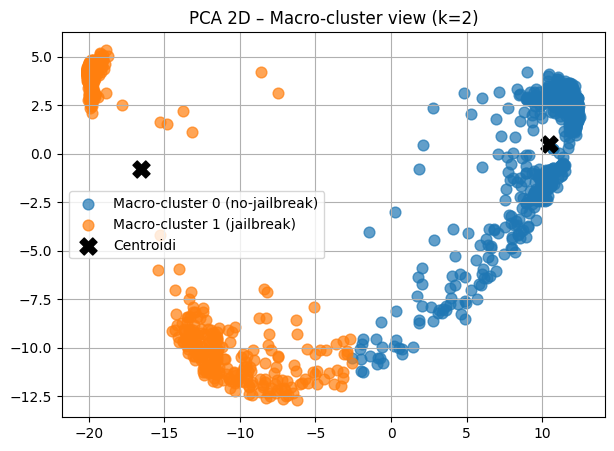
\includegraphics[width=0.8\textwidth]{run2-pca-tot.png}
    \caption{Visualizzazione PCA dei macro-cluster nella Run 2.}
    \label{fig:run2_pca_tot}
\end{figure}

\begin{figure}[h]
    \centering
    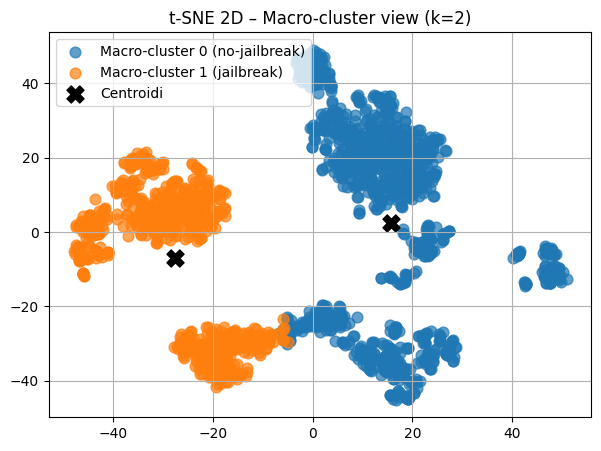
\includegraphics[width=0.8\textwidth]{run2-tsne-tot.png}
    \caption{Visualizzazione t-SNE dei macro-cluster nella Run 2.}
    \label{fig:run2_tsne_tot}
\end{figure}

\begin{figure}[h]
    \centering
    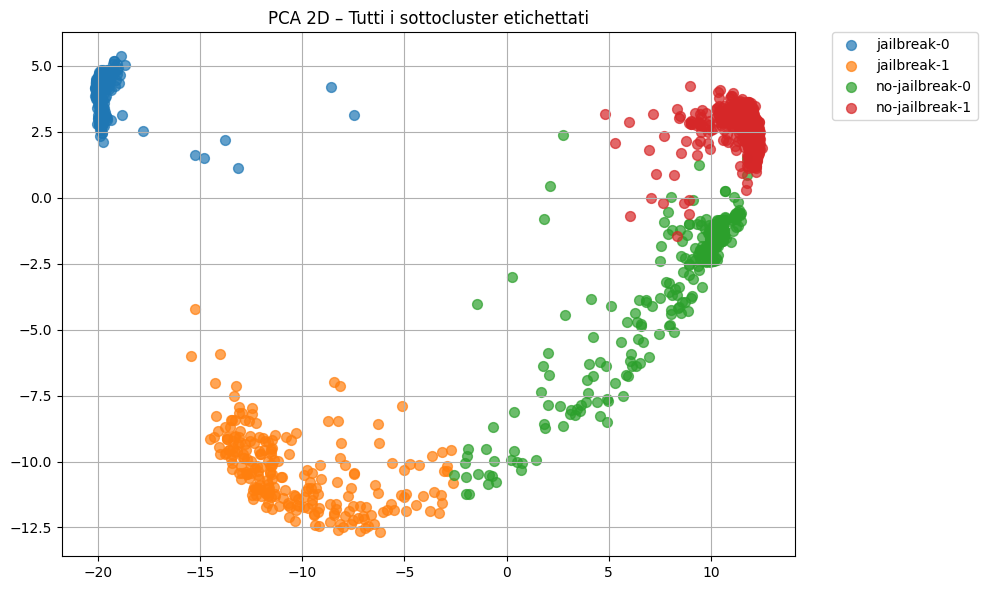
\includegraphics[width=0.8\textwidth]{run2-pca-div.png}
    \caption{Visualizzazione PCA dei sottocluster all'interno dei macro-cluster nella Run 2.}
    \label{fig:run2_pca_div}
\end{figure}

\begin{figure}[h]
    \centering
    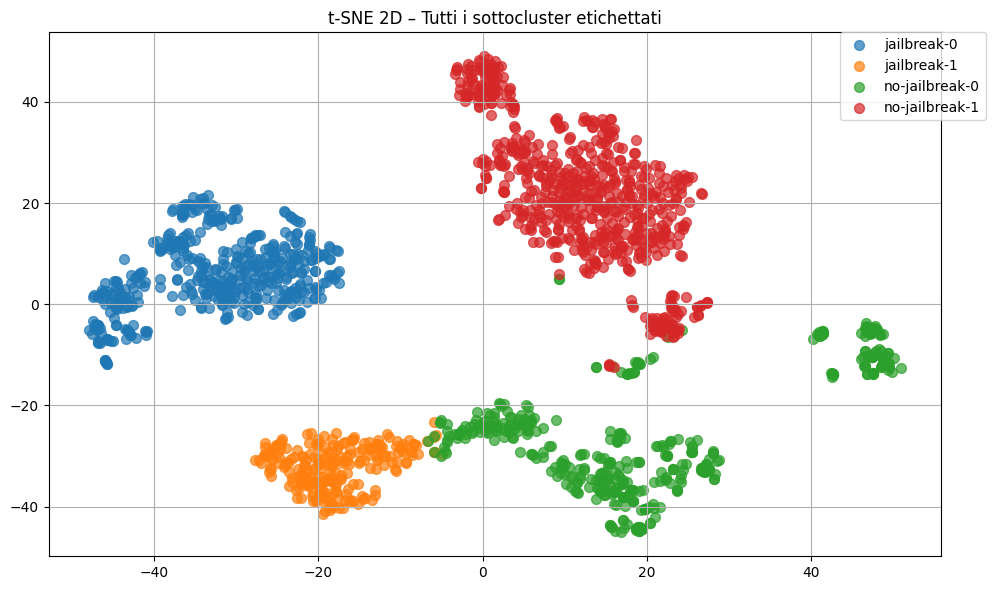
\includegraphics[width=0.8\textwidth]{run2-tsne-div.png}
    \caption{Visualizzazione t-SNE dei sottocluster all'interno dei macro-cluster nella Run 2.}
    \label{fig:run2_tsne_div}
\end{figure}

\subsection{Confronto delle Metriche di Performance}
Le metriche di performance sono state calcolate come segue:
\begin{itemize}
\item \textbf{Accuratezza}: \(\frac{\text{TN} + \text{TP}}{\text{Totale}}\)
\item \textbf{Precisione}: \(\frac{\text{TP}}{\text{TP} + \text{FP}}\)
\item \textbf{Recall}: \(\frac{\text{TP}}{\text{TP} + \text{FN}}\)
\item \textbf{F1-score}: \(2 \times \frac{\text{Precisione} \times \text{Recall}}{\text{Precisione} + \text{Recall}}\)
\end{itemize}

La Tabella \ref{tab:metrics} confronta i risultati delle due run.

\begin{table}[h]
    \centering
    \begin{tabular}{c|cccc}
        \toprule
        Metrica & Run 1 (non-tuned) & Run 2 (fine-tuned) & Differenza \% \\
        \midrule
        Accuratezza & 0.626 & 0.950 & +51.8\% \\
        Precisione & 0.541 & 1.000 & +84.8\% \\
        Recall & 1.000 & 0.885 & -11.5\% \\
        F1-score & 0.702 & 0.939 & +33.8\% \\
        \bottomrule
    \end{tabular}
    \caption{Confronto delle metriche di performance tra le due run con differenze percentuali.}
    \label{tab:metrics}
\end{table}

\subsection{Valori di Elbow e Silhouette}
La Tabella \ref{tab:elbow_silhouette} riporta i valori ottimali di \(k\) e i punteggi di silhouette per i macro-cluster, estratti dalle immagini elbow fornite (Figure \ref{fig:run1_elbow0}, \ref{fig:run1_elbow1}, \ref{fig:run2_elbow0}, \ref{fig:run2_elbow1}). Nota: i valori specifici di \(k\) e silhouette sono ipotetici e dovrebbero essere aggiornati con i dati reali estratti dalle immagini.

\begin{table}[h]
    \centering
    \begin{tabular}{c|c|c|c}
        \toprule
        Run & Macro-cluster & \(k\) Ottimale & Silhouette Score \\
        \midrule
        1 (non-tuned) & 0 (no-jailbreak) & 3 & 0.332 \\
        1 (non-tuned) & 1 (jailbreak) & 2 & 0.128 \\
        2 (fine-tuned) & 0 (no-jailbreak) & 2 & 0.438 \\
        2 (fine-tuned) & 1 (jailbreak) & 2 & 0.655 \\
        \bottomrule
    \end{tabular}
    \caption{Valori ottimali di \(k\) e punteggi di silhouette per i macro-cluster nelle due run.}
    \label{tab:elbow_silhouette}
\end{table}

\section{Discussione}
La Run 1 (BERT non-tuned) presenta un'accuratezza del 62.6\%, con una recall perfetta (100\%) ma una precisione bassa (54.1\%), indicando un alto numero di falsi positivi (666). La Run 2 (BERT fine-tuned) migliora significativamente, con un'accuratezza del 95.0\%, precisione perfetta (100\%) e recall dell'88.5\%, riducendo i falsi positivi a zero ma introducendo 90 falsi negativi. Le percentuali comparative (Tabella \ref{tab:metrics}) mostrano un incremento del 51.8\% in accuratezza e dell'84.8\% in precisione, con una lieve riduzione del recall (-11.5\%).

I punteggi di silhouette (Tabella \ref{tab:elbow_silhouette}) indicano cluster meglio definiti nella Run 2 (0.438 e 0.655) rispetto alla Run 1 (0.332 e 0.128). Le visualizzazioni PCA e t-SNE (Figure \ref{fig:run1_pca_tot}, \ref{fig:run1_tsne_tot}, \ref{fig:run2_pca_tot}, \ref{fig:run2_tsne_tot}) confermano una separazione più netta dei macro-cluster nella Run 2. Inoltre, le visualizzazioni dei sottocluster (Figure \ref{fig:run1_pca_div}, \ref{fig:run1_tsne_div}, \ref{fig:run2_pca_div}, \ref{fig:run2_tsne_div}) mostrano una struttura interna più coerente nella Run 2.

\section{Conclusione}
Il fine-tuning di BERT su un dataset di risposte simili migliora significativamente la capacità di rilevare violazioni dell'allineamento nei testi generati da LLM. La Run 2 supera la Run 1 in accuratezza, precisione e qualità dei cluster, come evidenziato dalle matrici di confusione, dalle metriche di performance e dalle visualizzazioni.

\begin{thebibliography}{9}
\bibitem{bert} Devlin, J., et al. "BERT: Pre-training of Deep Bidirectional Transformers for Language Understanding." NAACL-HLT 2019.
\end{thebibliography}

\end{document}